% Created by tikzDevice version 0.12 on 2019-04-13 14:06:16
% !TEX encoding = UTF-8 Unicode
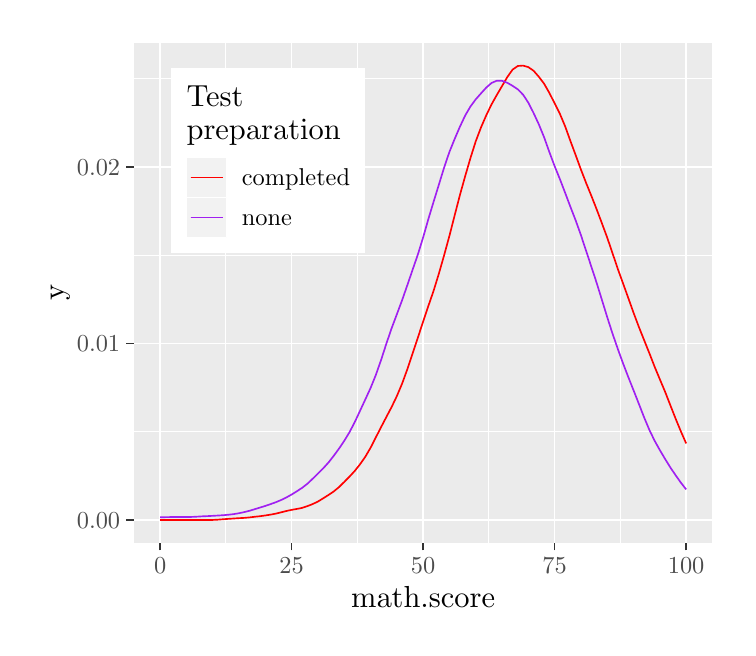
\begin{tikzpicture}[x=1pt,y=1pt]
\definecolor{fillColor}{RGB}{255,255,255}
\path[use as bounding box,fill=fillColor,fill opacity=0.00] (0,0) rectangle (252.94,216.81);
\begin{scope}
\path[clip] (  0.00,  0.00) rectangle (252.94,216.81);
\definecolor{drawColor}{RGB}{255,255,255}
\definecolor{fillColor}{RGB}{255,255,255}

\path[draw=drawColor,line width= 0.6pt,line join=round,line cap=round,fill=fillColor] (  0.00,  0.00) rectangle (252.94,216.81);
\end{scope}
\begin{scope}
\path[clip] ( 38.36, 30.72) rectangle (247.44,211.31);
\definecolor{fillColor}{gray}{0.92}

\path[fill=fillColor] ( 38.36, 30.72) rectangle (247.44,211.31);
\definecolor{drawColor}{RGB}{255,255,255}

\path[draw=drawColor,line width= 0.3pt,line join=round] ( 38.36, 70.82) --
	(247.44, 70.82);

\path[draw=drawColor,line width= 0.3pt,line join=round] ( 38.36,134.59) --
	(247.44,134.59);

\path[draw=drawColor,line width= 0.3pt,line join=round] ( 38.36,198.36) --
	(247.44,198.36);

\path[draw=drawColor,line width= 0.3pt,line join=round] ( 71.62, 30.72) --
	( 71.62,211.31);

\path[draw=drawColor,line width= 0.3pt,line join=round] (119.14, 30.72) --
	(119.14,211.31);

\path[draw=drawColor,line width= 0.3pt,line join=round] (166.66, 30.72) --
	(166.66,211.31);

\path[draw=drawColor,line width= 0.3pt,line join=round] (214.18, 30.72) --
	(214.18,211.31);

\path[draw=drawColor,line width= 0.6pt,line join=round] ( 38.36, 38.93) --
	(247.44, 38.93);

\path[draw=drawColor,line width= 0.6pt,line join=round] ( 38.36,102.70) --
	(247.44,102.70);

\path[draw=drawColor,line width= 0.6pt,line join=round] ( 38.36,166.47) --
	(247.44,166.47);

\path[draw=drawColor,line width= 0.6pt,line join=round] ( 47.86, 30.72) --
	( 47.86,211.31);

\path[draw=drawColor,line width= 0.6pt,line join=round] ( 95.38, 30.72) --
	( 95.38,211.31);

\path[draw=drawColor,line width= 0.6pt,line join=round] (142.90, 30.72) --
	(142.90,211.31);

\path[draw=drawColor,line width= 0.6pt,line join=round] (190.42, 30.72) --
	(190.42,211.31);

\path[draw=drawColor,line width= 0.6pt,line join=round] (237.94, 30.72) --
	(237.94,211.31);
\definecolor{drawColor}{RGB}{255,0,0}

\path[draw=drawColor,line width= 0.6pt,line join=round] ( 47.86, 38.93) --
	( 49.77, 38.93) --
	( 51.67, 38.93) --
	( 53.57, 38.93) --
	( 55.47, 38.93) --
	( 57.37, 38.93) --
	( 59.27, 38.93) --
	( 61.17, 38.93) --
	( 63.07, 38.93) --
	( 64.97, 38.93) --
	( 66.87, 38.93) --
	( 68.77, 39.03) --
	( 70.67, 39.18) --
	( 72.57, 39.32) --
	( 74.48, 39.45) --
	( 76.38, 39.57) --
	( 78.28, 39.67) --
	( 80.18, 39.85) --
	( 82.08, 40.08) --
	( 83.98, 40.28) --
	( 85.88, 40.55) --
	( 87.78, 40.85) --
	( 89.68, 41.21) --
	( 91.58, 41.68) --
	( 93.48, 42.16) --
	( 95.38, 42.57) --
	( 97.28, 42.91) --
	( 99.19, 43.28) --
	(101.09, 43.93) --
	(102.99, 44.67) --
	(104.89, 45.58) --
	(106.79, 46.74) --
	(108.69, 47.95) --
	(110.59, 49.22) --
	(112.49, 50.79) --
	(114.39, 52.66) --
	(116.29, 54.58) --
	(118.19, 56.64) --
	(120.09, 59.03) --
	(121.99, 61.74) --
	(123.90, 65.01) --
	(125.80, 68.75) --
	(127.70, 72.46) --
	(129.60, 76.11) --
	(131.50, 79.72) --
	(133.40, 83.67) --
	(135.30, 88.19) --
	(137.20, 93.42) --
	(139.10, 99.08) --
	(141.00,104.85) --
	(142.90,110.58) --
	(144.80,116.29) --
	(146.70,121.80) --
	(148.61,128.01) --
	(150.51,134.68) --
	(152.41,141.63) --
	(154.31,149.07) --
	(156.21,156.41) --
	(158.11,163.23) --
	(160.01,169.74) --
	(161.91,175.75) --
	(163.81,180.77) --
	(165.71,185.14) --
	(167.61,189.08) --
	(169.51,192.47) --
	(171.41,195.71) --
	(173.32,198.97) --
	(175.22,201.65) --
	(177.12,202.97) --
	(179.02,203.10) --
	(180.92,202.55) --
	(182.82,201.23) --
	(184.72,199.05) --
	(186.62,196.54) --
	(188.52,193.21) --
	(190.42,189.46) --
	(192.32,185.66) --
	(194.22,181.13) --
	(196.12,175.85) --
	(198.03,170.71) --
	(199.93,165.50) --
	(201.83,160.60) --
	(203.73,155.93) --
	(205.63,151.09) --
	(207.53,146.04) --
	(209.43,140.90) --
	(211.33,135.31) --
	(213.23,129.66) --
	(215.13,124.42) --
	(217.03,119.12) --
	(218.93,113.79) --
	(220.83,108.73) --
	(222.74,103.93) --
	(224.64, 99.20) --
	(226.54, 94.30) --
	(228.44, 89.73) --
	(230.34, 85.22) --
	(232.24, 80.34) --
	(234.14, 75.50) --
	(236.04, 70.91) --
	(237.94, 66.57);
\definecolor{drawColor}{RGB}{160,32,240}

\path[draw=drawColor,line width= 0.6pt,line join=round] ( 47.86, 39.88) --
	( 49.77, 39.93) --
	( 51.67, 39.97) --
	( 53.57, 40.00) --
	( 55.47, 40.00) --
	( 57.37, 40.00) --
	( 59.27, 40.02) --
	( 61.17, 40.11) --
	( 63.07, 40.23) --
	( 64.97, 40.31) --
	( 66.87, 40.41) --
	( 68.77, 40.52) --
	( 70.67, 40.64) --
	( 72.57, 40.81) --
	( 74.48, 41.04) --
	( 76.38, 41.36) --
	( 78.28, 41.77) --
	( 80.18, 42.24) --
	( 82.08, 42.83) --
	( 83.98, 43.41) --
	( 85.88, 43.99) --
	( 87.78, 44.65) --
	( 89.68, 45.33) --
	( 91.58, 46.13) --
	( 93.48, 47.06) --
	( 95.38, 48.11) --
	( 97.28, 49.29) --
	( 99.19, 50.54) --
	(101.09, 52.02) --
	(102.99, 53.82) --
	(104.89, 55.71) --
	(106.79, 57.58) --
	(108.69, 59.67) --
	(110.59, 62.09) --
	(112.49, 64.69) --
	(114.39, 67.51) --
	(116.29, 70.63) --
	(118.19, 74.28) --
	(120.09, 78.35) --
	(121.99, 82.44) --
	(123.90, 86.59) --
	(125.80, 91.29) --
	(127.70, 96.72) --
	(129.60,102.59) --
	(131.50,108.17) --
	(133.40,113.24) --
	(135.30,118.33) --
	(137.20,123.80) --
	(139.10,129.36) --
	(141.00,134.86) --
	(142.90,141.03) --
	(144.80,147.69) --
	(146.70,153.98) --
	(148.61,160.16) --
	(150.51,166.36) --
	(152.41,171.95) --
	(154.31,176.64) --
	(156.21,181.07) --
	(158.11,185.10) --
	(160.01,188.35) --
	(161.91,190.91) --
	(163.81,193.07) --
	(165.71,195.16) --
	(167.61,196.82) --
	(169.51,197.64) --
	(171.41,197.60) --
	(173.32,196.89) --
	(175.22,195.79) --
	(177.12,194.51) --
	(179.02,192.59) --
	(180.92,189.69) --
	(182.82,185.94) --
	(184.72,181.84) --
	(186.62,177.19) --
	(188.52,171.83) --
	(190.42,166.75) --
	(192.32,162.08) --
	(194.22,157.11) --
	(196.12,152.06) --
	(198.03,147.13) --
	(199.93,141.81) --
	(201.83,136.02) --
	(203.73,130.29) --
	(205.63,124.49) --
	(207.53,118.35) --
	(209.43,112.16) --
	(211.33,106.26) --
	(213.23,100.76) --
	(215.13, 95.52) --
	(217.03, 90.55) --
	(218.93, 85.78) --
	(220.83, 80.93) --
	(222.74, 76.01) --
	(224.64, 71.48) --
	(226.54, 67.55) --
	(228.44, 64.15) --
	(230.34, 60.94) --
	(232.24, 57.88) --
	(234.14, 55.06) --
	(236.04, 52.39) --
	(237.94, 49.96);
\end{scope}
\begin{scope}
\path[clip] (  0.00,  0.00) rectangle (252.94,216.81);
\definecolor{drawColor}{gray}{0.30}

\node[text=drawColor,anchor=base east,inner sep=0pt, outer sep=0pt, scale=  0.88] at ( 33.41, 35.90) {0.00};

\node[text=drawColor,anchor=base east,inner sep=0pt, outer sep=0pt, scale=  0.88] at ( 33.41, 99.67) {0.01};

\node[text=drawColor,anchor=base east,inner sep=0pt, outer sep=0pt, scale=  0.88] at ( 33.41,163.44) {0.02};
\end{scope}
\begin{scope}
\path[clip] (  0.00,  0.00) rectangle (252.94,216.81);
\definecolor{drawColor}{gray}{0.20}

\path[draw=drawColor,line width= 0.6pt,line join=round] ( 35.61, 38.93) --
	( 38.36, 38.93);

\path[draw=drawColor,line width= 0.6pt,line join=round] ( 35.61,102.70) --
	( 38.36,102.70);

\path[draw=drawColor,line width= 0.6pt,line join=round] ( 35.61,166.47) --
	( 38.36,166.47);
\end{scope}
\begin{scope}
\path[clip] (  0.00,  0.00) rectangle (252.94,216.81);
\definecolor{drawColor}{gray}{0.20}

\path[draw=drawColor,line width= 0.6pt,line join=round] ( 47.86, 27.97) --
	( 47.86, 30.72);

\path[draw=drawColor,line width= 0.6pt,line join=round] ( 95.38, 27.97) --
	( 95.38, 30.72);

\path[draw=drawColor,line width= 0.6pt,line join=round] (142.90, 27.97) --
	(142.90, 30.72);

\path[draw=drawColor,line width= 0.6pt,line join=round] (190.42, 27.97) --
	(190.42, 30.72);

\path[draw=drawColor,line width= 0.6pt,line join=round] (237.94, 27.97) --
	(237.94, 30.72);
\end{scope}
\begin{scope}
\path[clip] (  0.00,  0.00) rectangle (252.94,216.81);
\definecolor{drawColor}{gray}{0.30}

\node[text=drawColor,anchor=base,inner sep=0pt, outer sep=0pt, scale=  0.88] at ( 47.86, 19.71) {0};

\node[text=drawColor,anchor=base,inner sep=0pt, outer sep=0pt, scale=  0.88] at ( 95.38, 19.71) {25};

\node[text=drawColor,anchor=base,inner sep=0pt, outer sep=0pt, scale=  0.88] at (142.90, 19.71) {50};

\node[text=drawColor,anchor=base,inner sep=0pt, outer sep=0pt, scale=  0.88] at (190.42, 19.71) {75};

\node[text=drawColor,anchor=base,inner sep=0pt, outer sep=0pt, scale=  0.88] at (237.94, 19.71) {100};
\end{scope}
\begin{scope}
\path[clip] (  0.00,  0.00) rectangle (252.94,216.81);
\definecolor{drawColor}{RGB}{0,0,0}

\node[text=drawColor,anchor=base,inner sep=0pt, outer sep=0pt, scale=  1.10] at (142.90,  7.44) {math.score};
\end{scope}
\begin{scope}
\path[clip] (  0.00,  0.00) rectangle (252.94,216.81);
\definecolor{drawColor}{RGB}{0,0,0}

\node[text=drawColor,rotate= 90.00,anchor=base,inner sep=0pt, outer sep=0pt, scale=  1.10] at ( 13.08,121.02) {y};
\end{scope}
\begin{scope}
\path[clip] (  0.00,  0.00) rectangle (252.94,216.81);
\definecolor{fillColor}{RGB}{255,255,255}

\path[fill=fillColor] ( 51.94,135.47) rectangle (121.99,202.28);
\end{scope}
\begin{scope}
\path[clip] (  0.00,  0.00) rectangle (252.94,216.81);
\definecolor{drawColor}{RGB}{0,0,0}

\node[text=drawColor,anchor=base west,inner sep=0pt, outer sep=0pt, scale=  1.10] at ( 57.44,188.23) {Test };

\node[text=drawColor,anchor=base west,inner sep=0pt, outer sep=0pt, scale=  1.10] at ( 57.44,176.35) { preparation};
\end{scope}
\begin{scope}
\path[clip] (  0.00,  0.00) rectangle (252.94,216.81);
\definecolor{drawColor}{RGB}{255,255,255}
\definecolor{fillColor}{gray}{0.95}

\path[draw=drawColor,line width= 0.6pt,line join=round,line cap=round,fill=fillColor] ( 57.44,155.43) rectangle ( 71.89,169.88);
\end{scope}
\begin{scope}
\path[clip] (  0.00,  0.00) rectangle (252.94,216.81);
\definecolor{drawColor}{RGB}{255,0,0}

\path[draw=drawColor,line width= 0.6pt,line join=round] ( 58.88,162.65) -- ( 70.45,162.65);
\end{scope}
\begin{scope}
\path[clip] (  0.00,  0.00) rectangle (252.94,216.81);
\definecolor{drawColor}{RGB}{255,0,0}

\path[draw=drawColor,line width= 0.6pt,line join=round] ( 58.88,162.65) -- ( 70.45,162.65);
\end{scope}
\begin{scope}
\path[clip] (  0.00,  0.00) rectangle (252.94,216.81);
\definecolor{drawColor}{RGB}{255,255,255}
\definecolor{fillColor}{gray}{0.95}

\path[draw=drawColor,line width= 0.6pt,line join=round,line cap=round,fill=fillColor] ( 57.44,140.97) rectangle ( 71.89,155.43);
\end{scope}
\begin{scope}
\path[clip] (  0.00,  0.00) rectangle (252.94,216.81);
\definecolor{drawColor}{RGB}{160,32,240}

\path[draw=drawColor,line width= 0.6pt,line join=round] ( 58.88,148.20) -- ( 70.45,148.20);
\end{scope}
\begin{scope}
\path[clip] (  0.00,  0.00) rectangle (252.94,216.81);
\definecolor{drawColor}{RGB}{160,32,240}

\path[draw=drawColor,line width= 0.6pt,line join=round] ( 58.88,148.20) -- ( 70.45,148.20);
\end{scope}
\begin{scope}
\path[clip] (  0.00,  0.00) rectangle (252.94,216.81);
\definecolor{drawColor}{RGB}{0,0,0}

\node[text=drawColor,anchor=base west,inner sep=0pt, outer sep=0pt, scale=  0.88] at ( 77.39,159.62) {completed};
\end{scope}
\begin{scope}
\path[clip] (  0.00,  0.00) rectangle (252.94,216.81);
\definecolor{drawColor}{RGB}{0,0,0}

\node[text=drawColor,anchor=base west,inner sep=0pt, outer sep=0pt, scale=  0.88] at ( 77.39,145.17) {none};
\end{scope}
\end{tikzpicture}
